\chapter{Background}\label{background}

This chapter introduces the technological context in which this thesis was born with some references to the working environment in which it is implemented.

Since this document covers the workflow from designing application architecture in containers to deploying it in a real production environment, as well as using the application in development and QA environments, the context is presented from multiple points of view:

\begin{itemize}
\item the automation of the IT operations;
\item the evolution of the development workflow;
\item the scalability of architectures in the cloud;
\item the flexibility of multiple environments;
\item the key factors of Free Software and Sharing Economy that has led useful tools and practices used to develop the project.
\end{itemize}

\section{Manageability in IT
Operations}\label{manageability-in-it-operations}

Common GNU/Linux distributions comes with a built-in package manager
that provides a powerful entrypoint for installing and managing
packages, from libraries to graphical applications. Using this feature,
historically system administrators managed servers (IaaS)
manually directly via shell, upgrading the system, installing and
configuring the necessary packages. This approach introduces human
errors and non reproducible operations, so it's unsuitable when scaling
the numbers of engineers, hosts, applications and tasks. For example,
it's difficult updating all the configurations, because there is no formal way to do it.

Even if the manual management is immediate and doesn't need
preplanning, it has several limits. A first step derives from
other industrial revolutions, minimizing the human intervention and
\textit{automating} all operations as much as possible, via scripting or
dedicated tools for \textit{application deployment} and
\textit{configuration management} (e.g.: Chef\footnote{https://www.chef.io/chef/}, Puppet\footnote{https://puppetlabs.com/}, SaltStack\footnote{https://saltstack.com/community/},
Ansible\footnote{http://www.ansible.com/}). So humans doesn't do things directly, but instruct machines to
do it in a more efficient, reproducible and reliable way.  As described in \textit{Pets vs Cattle}\cite{PetsVsCattle}, while traditionally the server hostnames were chosen creatively as if they were cats, in an industrial approach these have to be chosen in a more pragmatic way as if they were cattle, for example with a semantic short name and a counter.

Even if this approach worked for years at scale, the application level
remains coupled to underlying infrastructure. In \textit{PaaS}, instead,
there is a clear separation of infrastructure and application levels.

From Wikipedia:

\begin{quote}
In the PaaS models, cloud providers deliver a computing platform,
typically including operating system, programming-language execution
environment, database, and web server. Application developers can
develop and run their software solutions on a cloud platform without the
cost and complexity of buying and managing the underlying hardware and
software layers. {[}\ldots{}{]}
\end{quote}

In 2009 \textit{Ian Murdock}, the Debian founder, in its article \textit{Do
operating systems still matter?}\cite{DoOperatingSystemsStillMatter}
concluded that today developers using a PaaS are not more concerned
about underlying hardware or operating system related features, but also
about platform-level exposed features, so operating systems should be
rethinked in order to expose a better, more integrated higher level
experience.

Also RedHat in \textit{The Platform Abstraction Advantage of
PaaS}\cite{ThePlatformAbstractionAdvantageOfPaaS} concludes with the
following:

\begin{quote}
Clearly, platform abstraction solves more problems for IT than an IaaS+
approach. Enterprises embrace cloud for agility benefits and having an
abstraction at the platform layer maximizes these benefits. DevOps is
more attractive for enterprises because their IT can now deliver at the
speed of business and the standardization of application development
platform through abstraction at higher layers of stack and self service
option for developers enables IT to meet the business needs.
\end{quote}

Table 2.1 and figure 2.1 show the evolution of IT Operations, from manual IaaS approach to a modern automated PaaS.

\begin{longtable}[c]{@{}lll@{}}
\caption{Summary of Evolution in IT Operations}\tabularnewline
\toprule
Model & Operations & IaaS/SaaS strong separation\tabularnewline
\midrule
\endfirsthead
\toprule
Model & Operations & IaaS/SaaS strong separation\tabularnewline
\midrule
\endhead
IaaS & manually & no\tabularnewline
IaaS+ & automated & no\tabularnewline
PaaS & automated & yes\tabularnewline
\bottomrule
\end{longtable}

\begin{figure}[htbp]
\centering
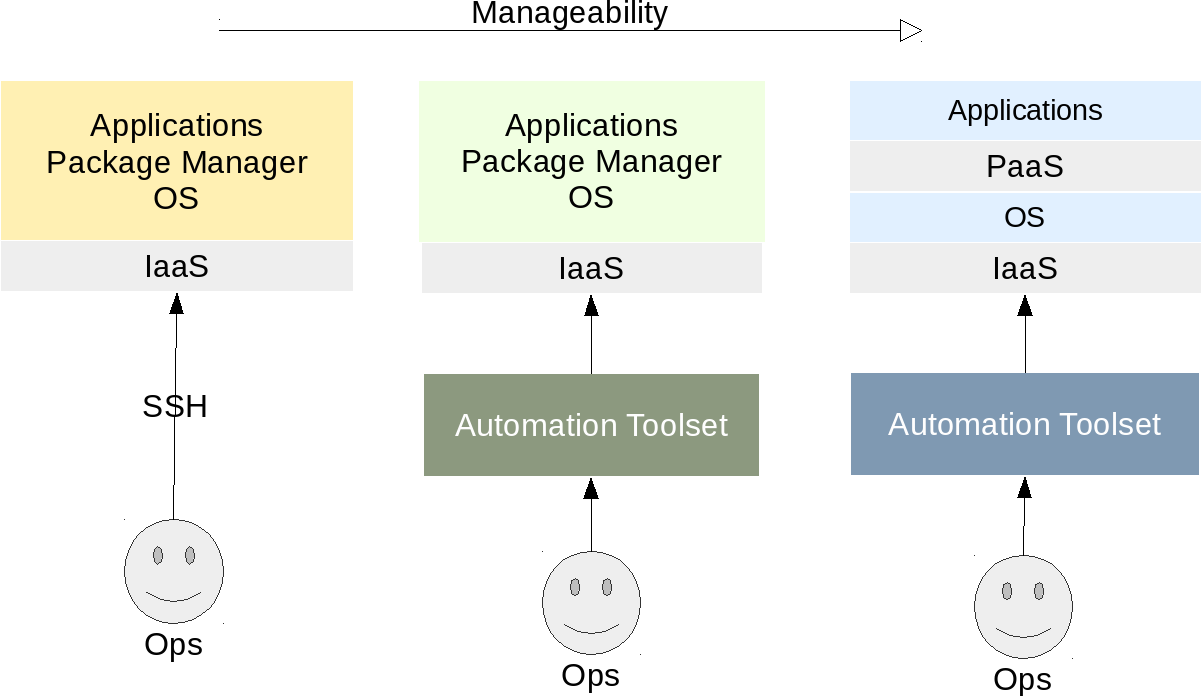
\includegraphics{media/ch2-paas.png}
\caption{Evolution in IT Operations}
\end{figure}

\section{Velocity in Development
Workflow}\label{velocity-in-development-workflow}

In 2001 was published the \textit{Agile Manifesto}\footnote{http://www.agilemanifesto.org/}, a set of 12 principles that represent a first step towards a faster and more efficient approach to developers needs, going beyond the traditional \textit{waterfall} development. From the development workflow point of view, agile practices introduced the \textit{Continuous Integration} (CI), a system in order to run tests automatically and notify to users when tests fail.

While Agile methodologies made the development faster, the users will not receive this since delivery of applications remains slow. That create the necessity for a more collaboration/interaction between development and operations/delivery teams in order to automating the application deployment as soon as it passed the tests. This is called Continuous Delivery\cite{ContinuousDelivery}, extending the CI concept to production.

Consequently, also development and production environment should getting close, aim to the so called \textit{dev/prod parity}. This way to build applications was formerly by Heroku, popular PaaS, with \textit{The
Twelve-Factor App}\cite{TheTwelveFactors}, a 12 good practices to apply
at SaaS:

\begin{enumerate}
\item Codebase:  One codebase tracked in revision control, many deploys
\item Dependencies:  Explicitly declare and isolate dependencies
\item Config: Store config in the environment
\item Backing Services:  Treat backing services as attached resources
\item Build, release, run:  Strictly separate build and run stages
\item Processes:  Execute the app as one or more stateless processes
\item Port binding:  Export services via port binding
\item Concurrency:  Scale out via the process model
\item Disposability:  Maximize robustness with fast startup and graceful shutdown
\item Dev/prod parity:  Keep development, staging, and production as similar as possible
\item Logs:  Treat logs as event streams
\item Admin processes:  Run admin/management tasks as one-off processes
\end{enumerate}

12factor separate clearly development and operations through a contract, and represent the beginning of DevOps era. Other PaaS shared and was born on top of these principles, such as Deis\footnote{http://deis.io/} or OpenShift.

In a DevOps context there are usually at least these components:

\begin{itemize}
\item \textit{Source Code Management} provides repositories hosting for Git   (or other source code versioning system) projects (e.g.: Gogs\footnote{http://gogs.io/},   GitLab\footnote{https://about.gitlab.com/});
\item \textit{Continuous Integration/Continuous Delivery} execute automated   tests and send somewhere else when software is ready to deploy in   staging, QA or production environment (e.g.: \textit{Travis CI},  GitLab CI\footnote{https://about.gitlab.com/gitlab-ci/}, Drone\footnote{https://drone.io/}, Jenkins\footnote{https://jenkins-ci.org/});
\item \textit{Platform as a Service} is the core of infrastructure and
  automatically manage the applications, including the upgrade, some
  monitoring features (e.g.: \textit{Deis}, \textit{OpenShift}).
\end{itemize}

Table 2.2 and figure 2.2 show the evolution in development workflow, from the traditional waterfall to the modern DevOps.

\begin{longtable}[c]{@{}lll@{}}
\caption{Summary of Evolution in Development Workflow}\tabularnewline
\toprule
Workflow & Development cycles & Delivery cycles\tabularnewline
\midrule
\endfirsthead
\toprule
Workflow & Development cycles & Delivery cycles\tabularnewline
\midrule
\endhead
Waterfall & long & long\tabularnewline
Agile & short (CI) & long\tabularnewline
DevOps & short (CI) & short (CD)\tabularnewline
\bottomrule
\end{longtable}

\begin{figure}[htbp]
\centering
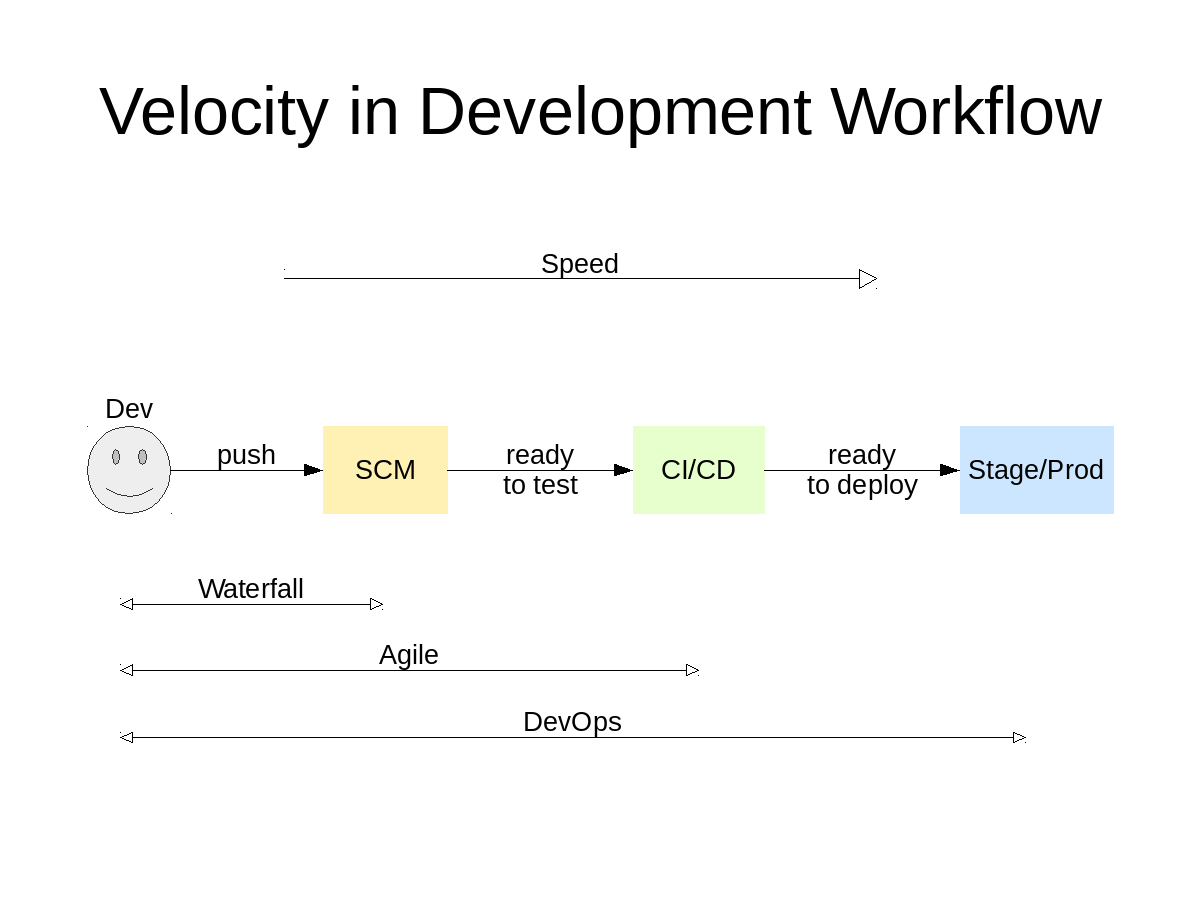
\includegraphics{media/ch2-devops.png}
\caption{Evolution of Development Workflow}
\end{figure}

\section{Scalability in Software
Architecture}\label{scalability-in-software-architecture}

The most common paradigm today is developing \textit{layered} applications
thanks to frameworks, like Django and Rails, that enables developers to
separate the various components, like data, business logic, routing,
templating, caching, etc. This approach has permitted for a better
manageability of spaghetti-code applications since it's possible to find
where is a particular piece of the application and enables scaling
through the layers, usually web/caching, application and database server
components.

While this lead several advantage, with increasing the sizing of
application, it could be to big making hard developing and scaling. The
\textit{microservices} pattern make the modularization another step, and
proposes loosely coupled, but independent applications that communicate
via APIs. This make possible use the best technology (language,
framework, database) for every specific need. Some of them could also be stateless for data processing only, without persistent storage capability.

Table 2.3 and figure 2.3 show the evolution of software architecture, from monolith application to a set of microservices.

\begin{longtable}[c]{@{}llll@{}}
\caption{Summary of Evolution in Software Architecture}\tabularnewline
\toprule
Architecture & Vertical Scaling & Horizontal Scaling & Data partitioning
Scaling\tabularnewline
\midrule
\endfirsthead
\toprule
Architecture & Vertical Scaling & Horizontal Scaling & Data partitioning
Scaling\tabularnewline
\midrule
\endhead
Monolith & yes & no & no\tabularnewline
Layered Monolith & yes & yes & no\tabularnewline
Microservices & yes & yes & yes\tabularnewline
\bottomrule
\end{longtable}

\begin{figure}[htbp]
\centering
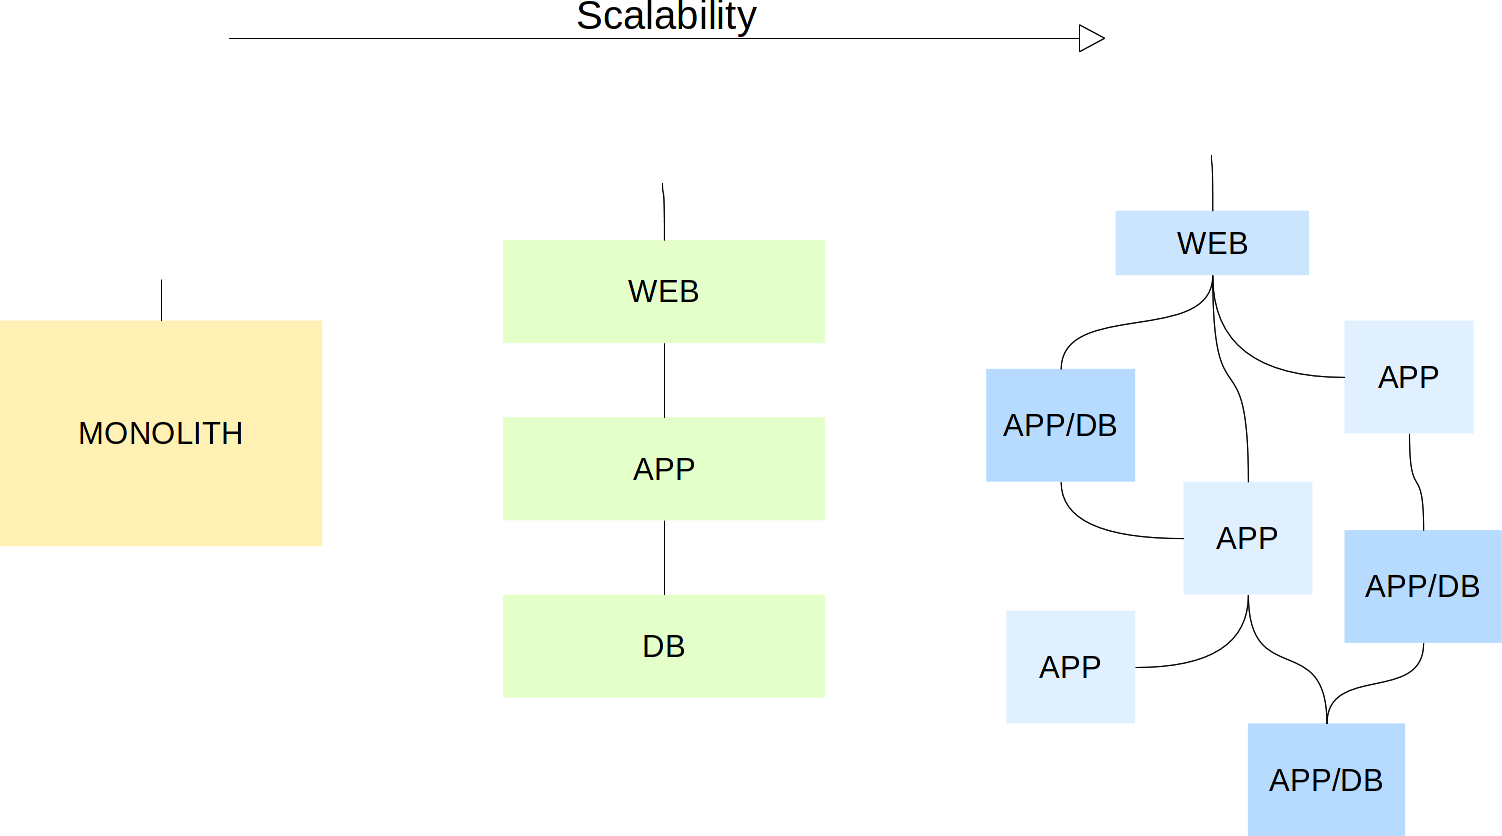
\includegraphics{media/ch2-microservices.png}
\caption{Evolution of Software Architectures}
\end{figure}

\section{Flexibility in Application
Environments}\label{flexibility-in-application-environments}

The final destination of every application is to be deployed somewhere
for producing an added-value for users/customers. Thanks to advantage in
terms of isolation and flexibility than \textit{physical machines}, today
\textit{virtual machines} (VM) represent the atom unit on which
applications are deployed. In fact, working on VMs is logically
equivalent, with a little of overhead.

At the beginning of 2013, was announced Docker, a \textit{container}
runtime (https://www.docker.com/whatisdocker) that aims to be the unit
of launching application components, running reproducible environments,
and conceived for developers friendly via Git-like CLI. Containers
doesn't offer all the isolation of VMs, but reduces the overhead and
permits to optimize resources.

Container technologies already exists, but historically were thought as
lightweight VMs in order to serve functional-complete operating systems.
Instead, Docker focused on deploying only single processes, separating
the OS from the application layers. Today containers, and Docker in
particular, are in full diffusion and it has been adopted by large
industry.

Table 2.4 and figure 2.4 show the evolution in application environments, from physical machines to containers.

\begin{longtable}[c]{@{}lll@{}}
\caption{Summary of Evolution in Application
Environments}\tabularnewline
\toprule
Environment & Hardware abstraction & Flexibility\tabularnewline
\midrule
\endfirsthead
\toprule
Environment & Hardware abstraction & Flexibility\tabularnewline
\midrule
\endhead
Physical Machines & no & no\tabularnewline
Virtual Machines & yes & low\tabularnewline
Containers & yes & high\tabularnewline
\bottomrule
\end{longtable}

\begin{figure}[htbp]
\centering
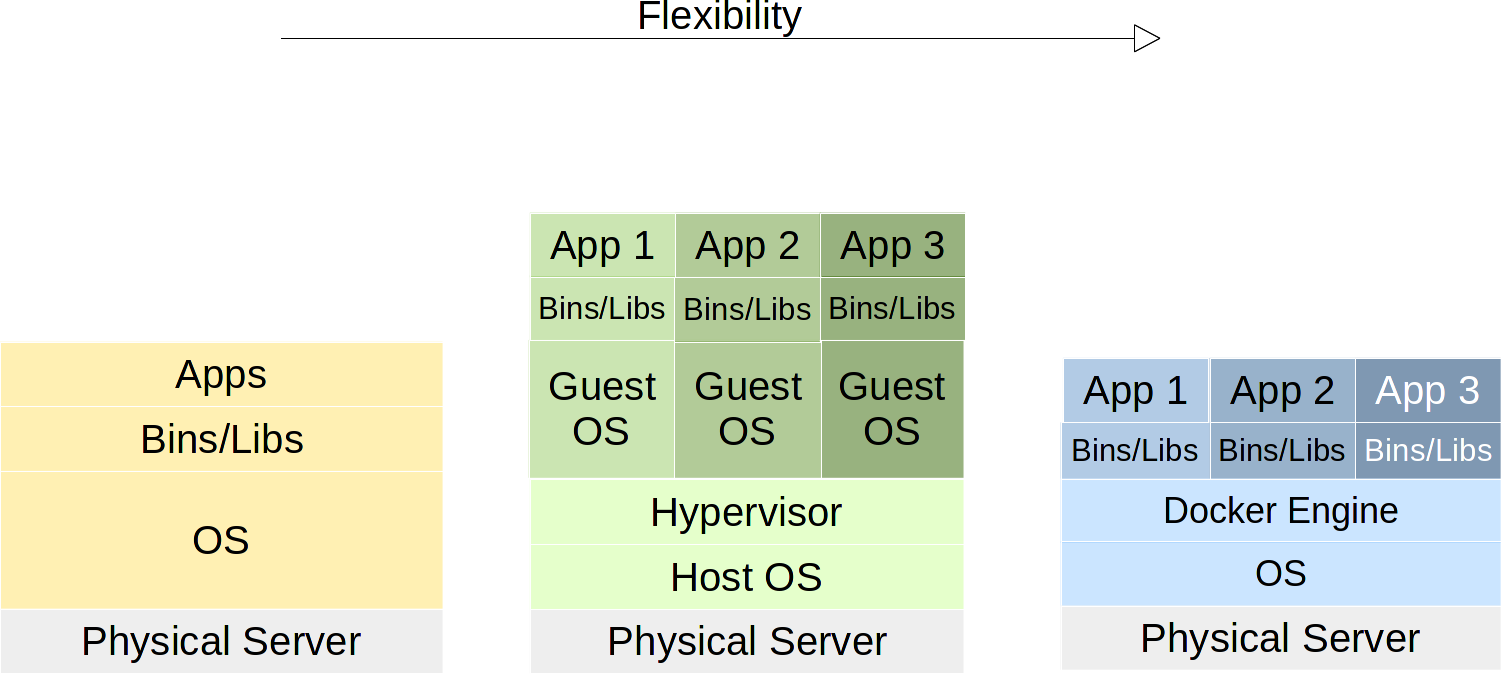
\includegraphics{media/ch2-containers.png}
\caption{Evolution of Application Environments}
\end{figure}

\section{Key Factors: Free Software and Sharing
Economy}\label{key-factors-free-software-and-sharing-economy}

In February 1986 Richard Matthew Stallman\footnote{https://www.stallman.org/} formalized\footnote{https://www.gnu.org/bulletins/bull1.txt} the first formal definition of Free Software in Free Software Foundation\footnote{https://fsf.org/} (FSF).  Then, the definition has been updated several times, and it's still maintained from FSF.  Shortly, depends on that Free Software definition\cite{FreeSoftwareDefinition}, a program is free software if the program's users have the four essential freedoms:

\begin{itemize}
\item The freedom to run the program as you wish, for any purpose (freedom 0).
\item The freedom to study how the program works, and change it so it does your computing as you wish (freedom 1). Access to the source code is a precondition for this.
\item The freedom to redistribute copies so you can help your neighbor (freedom 2).
\item The freedom to distribute copies of your modified versions to others (freedom 3). By doing this you can give the whole community a chance to benefit from your changes. Access to the source code is a precondition for this.
\end{itemize}

Free Software enables the opportunities of:

\begin{itemize}
\item keeping control over the software;
\item learning from other design choices and code implementation;
\item improving the software with bug-fixing and feature integration;
\item optimizing costs with working on shared projects;
\item obtain higher quality.
\end{itemize}

Free Software enables reuse and leverages the solutions, and enables rapid feedbacks lowering the "time to release". In the web and cloud age, Free Software gained a significant role and is everywhere. It's a key on which many companies and services rely their trust.

The Sharing Economy\footnote{http://www.thepeoplewhoshare.com/blog/what-is-the-sharing-economy} focuses on relations (a major interaction between providers and consumers), enhances the community, creates discussion places, and makes easier direct feedbacks. The Sharing Economy identifies a collaborative economy, based on cooperation. The Free Software fits very well in the Sharing Economy for the Information
Technology topics since it avoid lock-in and other restrictive/bad practices of traditional economy, that aim to centralization instead of distribution and collaboration.

\section{Case of Study: beFair and Gasista
Felice}\label{case-of-study-befair-and-gasista-felice}

\textit{Gasista Felice} is the main project developed by \textit{beFair}, a
small team involved in the \textit{Free Software} and \textit{Sharing
Economy} networks. beFair is the working environment thanks to which it
has been possible this thesis project.

Gasista Felice is a web platform to manage economy for solidarity-based
purchasing groups (GAS) and suppliers involved in Solidarity-based
economy districts (DES). They all practice Sharing Economy.

The currently production version of Gasista Felice is a web application
built on MVC framework with Python\footnote{https://www.python.org/} 2.7, Django\footnote{https://www.djangoproject.com/} 1.3 and PostgreSQL\footnote{http://www.postgresql.org/}, with
non-REST APIs and a frontend in JS/jQuery\footnote{https://jquery.com/}. The work is on a development
version with Python and Django 1.7, PostgreSQL, REST APIs and frontend
in AngularJS\footnote{https://angularjs.org/} and Bootstrap\footnote{http://getbootstrap.com/}.

\section{A Solution for Current State of
Art}\label{a-solution-for-current-state-of-art}

The figure 2.5 represents a possible summary of the IT evolution in last decades from multiple point of views.

\begin{longtable}[c]{@{}llll@{}}
\caption{Summary of Evolution in IT}\tabularnewline
\toprule
& 1990's & 2000's & 2010's\tabularnewline
\midrule
\endfirsthead
\toprule
& 1990's & 2000's & 2010's\tabularnewline
\midrule
\endhead
\textit{Development Workflow} & Waterfall & Agile & DevOps\tabularnewline
\textit{IT Operations} & IaaS & IaaS+ & PaaS\tabularnewline
\textit{Software Architecture} & Monolith & Layered Monolith &
Microservices\tabularnewline
\textit{Application Environment} & Physical Machines & Virtual Machines &
Containers\tabularnewline
\bottomrule
\end{longtable}

The solution provided is a Proof of Concept (PoC), thought beyond academic purpose for future real use, of a pre-configured free/libre toolset that enables IT operators to build a PaaS on top of a IaaS/cloud infrastructure, who aims to be optimal for scaling microservices, and DevOps-oriented via CD and container as the atomic unit.

Has been follow some guidelines:

\begin{itemize}
\item elasticity;
\item lightweight (should not occupy too much resources, compiled languages
  over interpreted ones);
\item reuse pre-existent components (don't reinvent the wheel);
\item reuse pre-existent network layers (avoid dedicated transport layer via agents/daemons, to install/configure/manage/update, and more surface attack);
\item composable pieces with simple interface over monolith;
\item convention over configuration: by default it should works (quite)  out-of-the-box, but remain customizable (low entry wall);
\item automation everywhere possible, few manual commands to install/deploy;
\item avoid tools requires programming language or custom syntax for configuration
\item stay on shoulders of giants (avoid too small community and risk to adopt tools without a solid/active contributor community);
\item minimize external dependencies;
\item low dependency from IaaS for (future) private cloud.
\end{itemize}

There are recent similar projects that should be quoted for completeness:

\begin{itemize}
\item Apollo\footnote{https://github.com/Capgemini/Apollo} from Capgemini, an open-source platform for   apps, microservices and big data. It consists of Mesos cluster   provisioning and orchestration using Packer\footnote{https://packer.io/} and Terraform;
\item MANTL\footnote{https://github.com/CiscoCloud/microservices-infrastructure} from Cisco Cloud, formerly \textit{Microservices Infrastructure}, is a modern platform for rapidly   deploying globally distributed services.
\end{itemize}

With these goals in mind, the following toolset has been chosen:

\begin{itemize}
\item Terraform: Infrastructure Provisioning
\item Docker Engine: Container Runtime
\item CoreOS: GNU/Linux distribution for containers
\item Kubernetes: Container Cluster Orchestration
\item OpenShift v3: PaaS for modern workflow
\end{itemize}

Figure 2.5 shows the current state of art on left side, and the proposed solution on the right side, covering from IaaS to SaaS abstraction levels.

\begin{figure}[htbp]
\centering
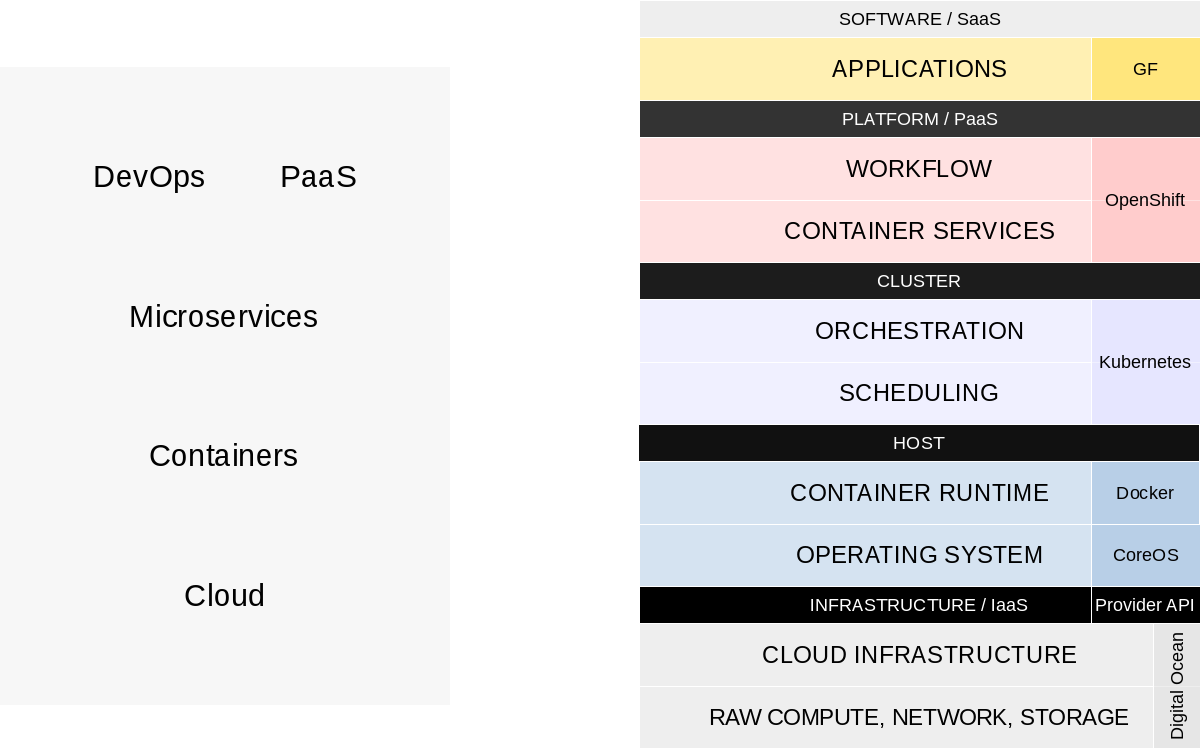
\includegraphics{media/ch2-solution.png}
\caption{From current state of art to a modern solution}
\end{figure}